\documentclass{exam}

\usepackage{units} 
\usepackage{graphicx}
\usepackage[fleqn]{amsmath}
\usepackage{cancel}
\usepackage{float}
\usepackage{mdwlist}
\usepackage{booktabs}
\usepackage{cancel}
\usepackage{polynom}
\usepackage{caption}
\usepackage{fullpage}
\usepackage{xfrac}
\usepackage{enumerate}

\newcommand{\degree}{\ensuremath{^\circ}} 
\everymath{\displaystyle}

\printanswers

% \begin{figure}[H]
%   \centering
%   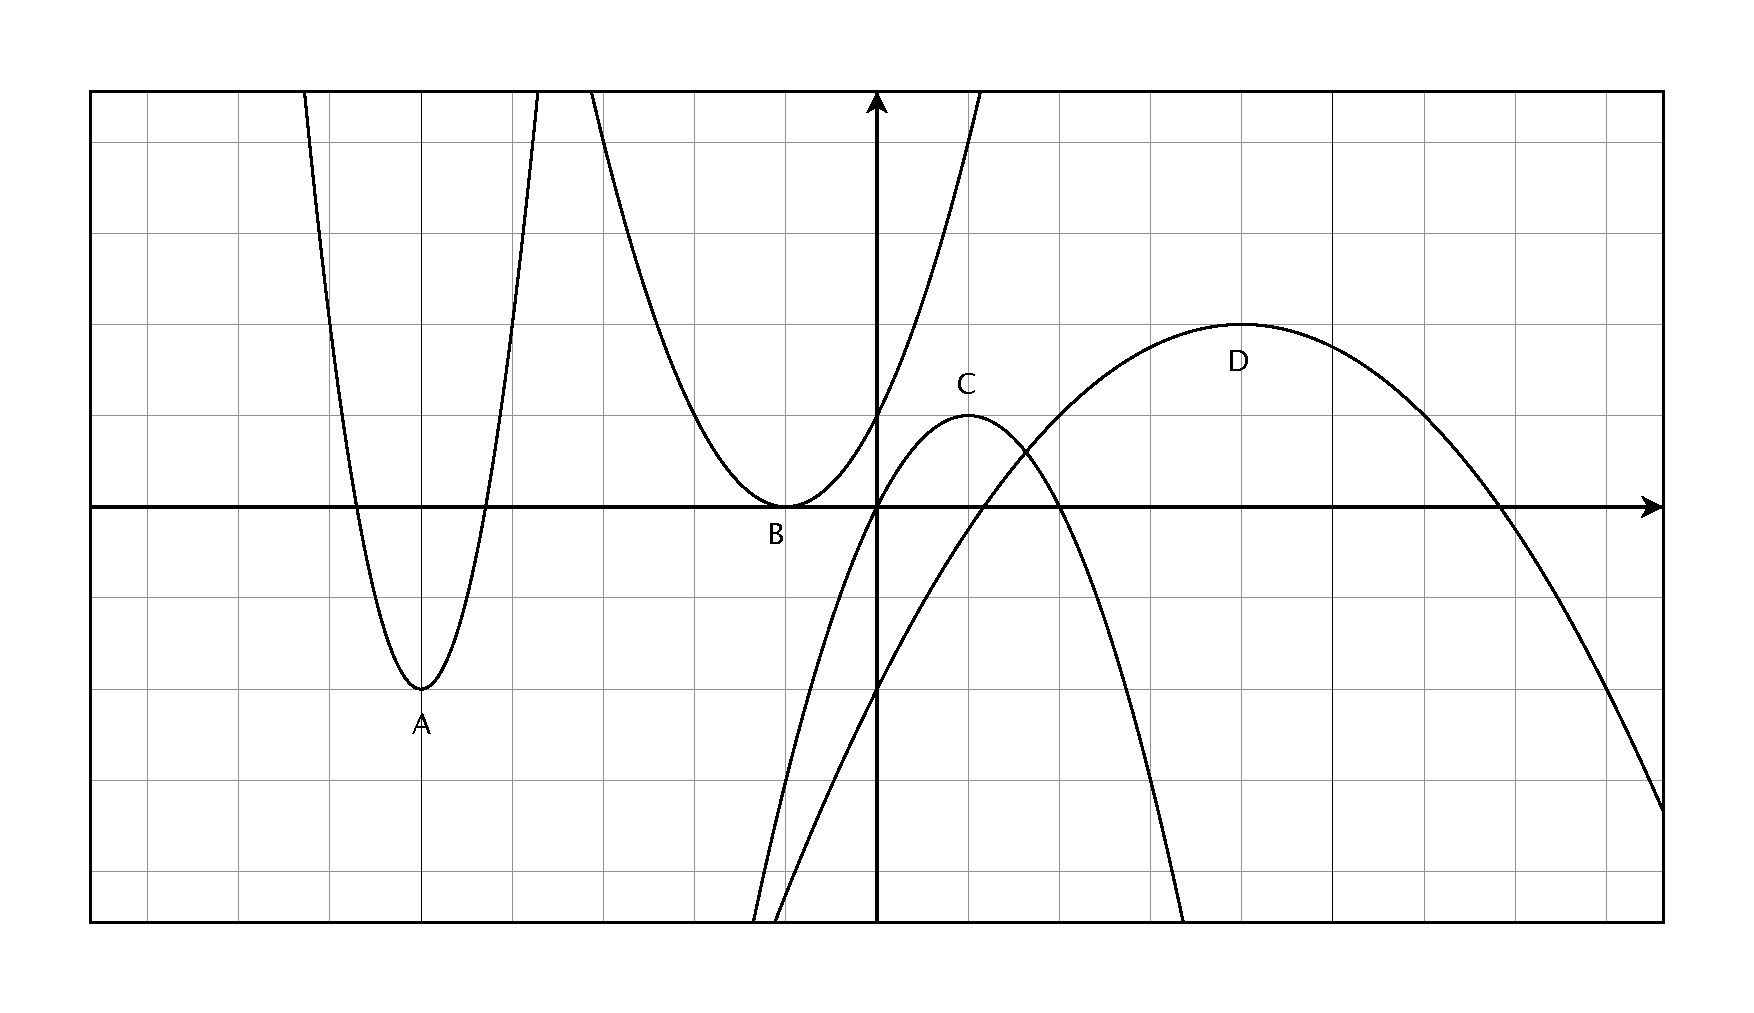
\includegraphics[scale=.3]{problem_7.eps}
%   \caption*{Problem 7}
% \end{figure}

% \begin{tabular}{cc}
% \toprule
% period & amplitude \\
% \midrule
%   $\pi$ & $2$ \\
% \bottomrule
% \end{tabular}

\title{Math 142 Notes \\ Section 5.1}

\date{\today}

\begin{document}

  \maketitle
  \tableofcontents

  \section{Unit Circle}

  \subsection{Description}
  \begin{itemize*}
    \item circle with radius one centered at origin.
    \item points on unit circle satisfy $x^2 + y^2 = 1$
  \end{itemize*}

  \subsection{Verifying Points}
  Verify following points are on unit circle:
  \begin{itemize*}
    \item $(1, 0)$
    \item $(0, 1)$
    \item $\left( \frac{\sqrt{2}}{2}, \frac{\sqrt{2}}{2} \right)$
    \item $\left( \frac{1}{3}, - \frac{2 \sqrt{2}}{3} \right)$
  \end{itemize*}

  \subsection{Finding Points}
  
  To find points given an x or y coordinate and a quadrant:
  \begin{itemize*}
    \item solve $x^2 + y^2 = 1$ for missing coordinate
    \item choose sign which puts point in correct quadrant
  \end{itemize*}

  \begin{itemize}
    \item $\left( x, \frac{1}{2} \right)$, quadrant II
    \item $\left( -\frac{3}{4}, y \right)$, quadrant III
    \item etc.
  \end{itemize}

  \section{Terminal Points}

  \subsection{Description}
  For terminal point determined by $t$, start at $(1, 0)$ and go counter-clockwise around unit circle distance $t$.  The
  point you reach is the terminal point for $t$.

  For negative $t$, go clockwise.

  \subsection{Examples}
  \begin{itemize}
    \item $\pi$, $2 \pi$, $\frac{\pi}{2}$, $-\pi$, $-\frac{3 \pi}{2}$, $8 \pi$, etc.
    \item $P = \left( \frac{1}{3}, \frac{\sqrt{6}}{3} \right)$, find terminal points for:
      \begin{enumerate}[a]
        \item $t + \pi$
        \item $-t$
        \item $\pi - t$
        \item $2 \pi + t$
      \end{enumerate}
  \end{itemize}

  \subsection{Interesting Points}

  \begin{itemize}
    \item $\frac{\pi}{4}$ is half way between $(1, 0)$ and $(0, 1)$, so $y = x$ and point is 
      $\left( \frac{\sqrt{2}}{2}, \frac{\sqrt{2}}{2} \right)$

    \item Draw equilateral triangle with side length one and one side on x-axis to find terminal point for
      $\frac{\pi}{3}$ is $\left( \frac{1}{2}, \frac{\sqrt{3}}{2} \right)$.

      Draw three equilateral triangles, with middle one upside down, all three inscribed in unit circle to demonstrate
      that angle is \sfrac{1}{3} of a circle.  

    \item Same figure with triangles along y-axis to find terminal point for $\frac{\pi}{6}$ 
      is $\left( \frac{1}{2}, \frac{\sqrt{3}}{2} \right)$

    \item Show same points in other quadrants

  \end{itemize}

  \section{Reference Number}
  \subsection{Description}
  Distance from x-axis determines absolute value of coordinates of terminal points.  Quadrant determines sign.  The
  ``reference number'' is the shortest distance along unit circle from x-axis to point.

  To find the reference number:
  \begin{itemize*}
    \item subtract suitable multiple of $\pi$
    \item take absolute value
  \end{itemize*}

  \subsection{Examples}
  Find reference number for $\frac{\pi}{3}$, $- \frac{\pi}{3}$, $\frac{2 \pi}{3}$, $\frac{7 \pi}{3}$, etc.


\end{document}
